\documentclass[oldfontcommands]{ucbthesis}
% General
\usepackage{lipsum}
\usepackage[at]{easylist}% easy lists with @ starting each item
\usepackage[usenames, dvipsnames]{color}
\usepackage{algorithm2e}

% Storage Sizing
\usepackage{lineno,hyperref}  % Line numbering
\usepackage{longtable}
\usepackage{amssymb}
\usepackage{amsmath}
\usepackage{textgreek}   % Non-italic greek symbols

% PowerMEMS
\usepackage{mathtools, capt-of}

% Strategic Equilibrium
\usepackage{amsfonts}

% Fully-decentralized security
\usepackage{amsmath, amssymb, amsfonts, subfig}
\usepackage{tikz}
\usetikzlibrary{positioning}

% Blockchain Microgrids
\usepackage{csquotes}
%\usepackage[usenames, dvipsnames]{color}
%\usepackage{algorithm2e}

\usepackage{tikz}
\usetikzlibrary{positioning}

%\usepackage{pstricks}
%\usepackage{graphics} % for pdf, bitmapped graphics files
\usepackage{graphicx} % for pdf, bitmapped graphics files
\usepackage{epsfig} % for postscript graphics files
%\usepackage{mathptmx} % assumes new font selection scheme installed
%\usepackage{times} % assumes new font selection scheme installed
\usepackage{amsmath} % assumes amsmath package installed
\usepackage{amssymb}  % assumes amsmath package installed
\usepackage{cite}
%\usepackage{flushend}
\usepackage{dsfont}
\usepackage{array}
\usepackage{lmodern}
\usepackage{float}

\usepackage{color,soul} %highlight text in yellow use commands \hl{}, 
\soulregister\cite7
\soulregister\ref7
\soulregister\pageref7

\newif\ifarticle \articlefalse
% Double spacing, if you want it.
% \def\dsp{\def\baselinestretch{2.0}\large\normalsize}
% \dsp

% If the Grad. Division insists that the first paragraph of a section
% be indented (like the others), then include this line:
% \usepackage{indentfirst}

%%%%%%%%%%%%%%%%%%
% If you want to use "sections" to partition your thesis
% un-comment the following:
% 
% \counterwithout{section}{chapter}
% \setsecnumdepth{subsubsection}
% \def\sectionmark#1{\markboth{#1}{#1}}
% \def\subsectionmark#1{\markboth{#1}{#1}}
% \renewcommand{\thesection}{\arabic{section}}
% \renewcommand{\thesubsection}{\thesection.\arabic{subsection}}
% \makeatletter
% \let\l@subsection\l@section
% \let\l@section\l@chapter
% \makeatother
% 
% \renewcommand{\thetable}{\arabic{table}}
% \renewcommand{\thefigure}{\arabic{figure}}
%
%%%%%%%%%%%%%%%%%%

%%\newtheorem{theorem}{Gibberish}
%%\hyphenation{mar-gin-al-ia}

\begin{document}

% Declarations for Front Matter

\title{Example Dissertation Using Modular LaTeX}
\author{Eric Munsing}
\degreesemester{Summer}
\degreeyear{2018}
\degree{Doctor of Philosophy}
\chair{Assistant Professor Scott J. Moura}
\othermembers{Professor Art Rosenfeld\\
	Professor Richard Feynman}
\numberofmembers{3}
\prevdegrees{B.S.M.E. (Franklin W. Olin College of Engineering) 2008 \\
  M.S. (University of California at Berkeley) 2014}
\field{Engineering - Civil and Environmental Engineering}
\campus{Berkeley}

\maketitle

%\approvalpage
% ^^ comment this out when compiling your final draft

\copyrightpage

\begin{abstract}
	\lipsum[4]

\begin{itemize}
	\item Chapter \ref{chap:background} provides background on the technical challenges of this work.
	\item Chapter \ref{chap:blockchains} Develops a novel approach to solving important problems.
	\item The Appendices present tutorial material on the tools used throughout the paper, and are supplemented by the code in the author's github repository: \texttt{\url{https://github.com/emunsing/tutorials}}
\end{itemize}

\lipsum[5-6]
\end{abstract}

\begin{frontmatter}

\begin{dedication}
\null\vfil
\begin{center}
To @ShitAcademicsSay\\\vspace{12pt}
For keeping me sane in the midst of the impossible
\end{center}
\vfil\null
\end{dedication}

\tableofcontents
\clearpage
\listoffigures
\clearpage
\listoftables

\begin{acknowledgements}
I would like to thank my arms for always being on my side, my legs for always supporting me, and my fingers because I can always count on them.
\end{acknowledgements}

\end{frontmatter}

\pagestyle{headings}

% (Optional) \part{First Part}

%% NOTE: In general I am using Git to sync individual articles to a local folder. In each of the articles, I am using the content.tex file to hold all the content (except the abstract).
%% The \makeatletter..\makeatother block assigns the local path for that context to look in the specific folder for that chapter, in order to not have to re-assign the graphics and input files.

\chapter{Background and Motivation}\label{chap:background}
\lipsum[1-4]
\makeatletter
\def\input@path{{chapters/background/}}
\def\Ginput@path{{chapters/background/}}
\makeatother
\section{Introduction}
\lipsum[1]

\subsection{Prior Literature}

As discussed in \cite{Eyer2010a,Sioshansi2012,Denholm2013,Makarov2012}, the findings from \cite{Walawalkar2007,Sioshansi2009} are clearly refuted. 
\lipsum[66]

This is in contrast with the methods of \cite{Kazempour2009,Kirby2012}, and the conventional modeling of \cite{EnergyandEnvironmentalEconomicsE32014a,Eyer2010a,Dunn2011,DepartmentofEnergy}. \lipsum[55]

%%%%%%%%%% SECTION

\section{Formulation}

\lipsum[5]

\begin{tabular}{c l}
$k$ 					& Time index, from 0 to time horizon $N$ \\
$\Delta t$ 				& Time step size (hours) \\
$c(k)$					& Energy flow into the battery at time $k$ (kW) \\
$d(k)$					& Energy flow out of the battery at time $k$ (kW) \\
$\text{P}_{\text{charge}}$		& Maximum charge power capacity of the system (kW) \\
$\text{P}_{\text{discharge}}$	& Maximum discharge power capacity of the system (kW) \\
$\text{c}_{\text{grid}}(k)$	& Nodal electricity clearing price (\$/kWh) \\
$\text{\texteta}_{\text{in}}$		& One-way system efficiency when charging \\ 
$\text{\texteta}_{\text{out}}$		& One-way system efficiency when discharging \\
$E(k)$					& Energy level in reservoir at time k \\
$\text{E}_{\min}$				& Minimum allowable energy level as portion of capacity \\
$\text{E}_{\max}$				& Maximum allowable energy level as portion of capacity \\
$\text{E}_{\text{init}}$		& Starting energy level of the storage system \\
$h$						& Reservoir capacity (h), in hours of peak discharge \\
$\text{\textgamma}$				& Annualized cost of constructing one kWh of reservoir capacity (\$/kWh/yr)
\end{tabular}


\subsection{Data}
\lipsum[2] As clearly demonstrated in Figure \ref{fig:datamap}

\begin{figure}
\centering
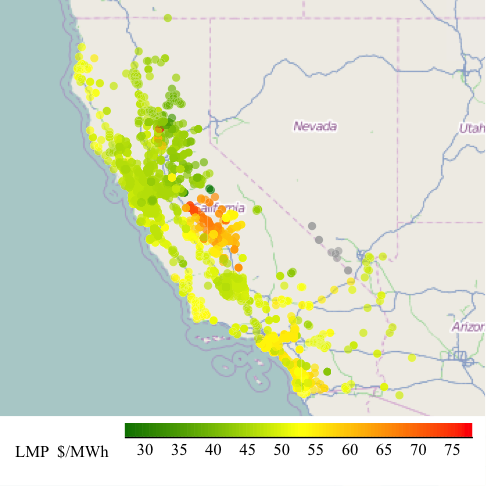
\includegraphics[trim = 0mm 0mm 0mm 0mm, clip, width=0.6\textwidth]{Figures/unprocessed_LMP_map.png}
\caption{Example of Location Marginal Price (LMP) distribution on the CAISO grid. Each circle represents an LMP node on the the CAISO grid. Data from 4PM PDT, August 18 2013}
\label{fig:datamap}
\end{figure}

\section{Results}
In Fig. \ref{fig:chargesize}, \lipsum[66]

\begin{figure}
\centering
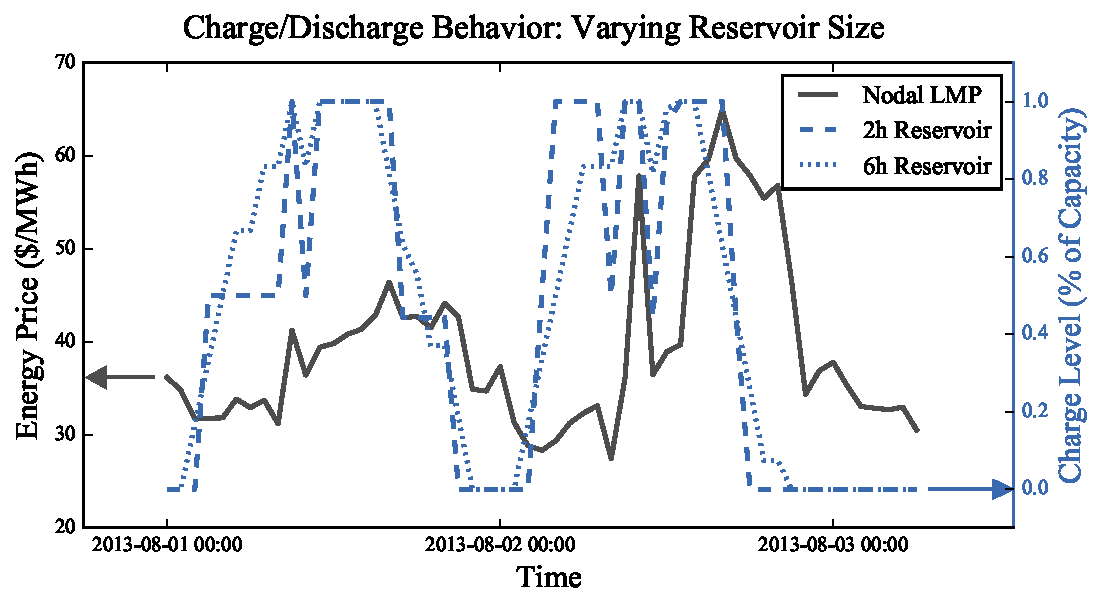
\includegraphics[trim = 0mm 0mm 0mm 0mm, clip, width=0.8\textwidth]{Figures/chargeValidation_varyingSize}
\caption{ Aenean massa. Cum sociis natoque penatibus et magnis dis parturient montes, nascetur ridiculus mus. Donec quam felis, ultricies nec, pellentesque eu, pretium quis, sem. Nulla consequat massa quis enim. }
\label{fig:chargesize}
\end{figure}

\lipsum[2-3]

%%%%%%%%%% CONCLUSION

\section{Conclusion}
\lipsum[22]

\section{Potential Improvements}
\lipsum[5-8]

%%---------------

\chapter{Blockchain-Coordinated Decentralized Optimization}\label{chap:blockchains}
\lipsum[1-4]
\makeatletter
\def\input@path{{chapters/blockchains/}}
\def\Ginput@path{{chapters/blockchains/}}
\makeatother
\section{Introduction}
\lipsum[1]

\subsection{Prior Literature}

As discussed in \cite{Eyer2010a,Sioshansi2012,Denholm2013,Makarov2012}, the findings from \cite{Walawalkar2007,Sioshansi2009} are clearly refuted. 
\lipsum[66]

This is in contrast with the methods of \cite{Kazempour2009,Kirby2012}, and the conventional modeling of \cite{EnergyandEnvironmentalEconomicsE32014a,Eyer2010a,Dunn2011,DepartmentofEnergy}. \lipsum[55]

%%%%%%%%%% SECTION

\section{Formulation}

\lipsum[5]

\begin{tabular}{c l}
$k$ 					& Time index, from 0 to time horizon $N$ \\
$\Delta t$ 				& Time step size (hours) \\
$c(k)$					& Energy flow into the battery at time $k$ (kW) \\
$d(k)$					& Energy flow out of the battery at time $k$ (kW) \\
$\text{P}_{\text{charge}}$		& Maximum charge power capacity of the system (kW) \\
$\text{P}_{\text{discharge}}$	& Maximum discharge power capacity of the system (kW) \\
$\text{c}_{\text{grid}}(k)$	& Nodal electricity clearing price (\$/kWh) \\
$\text{\texteta}_{\text{in}}$		& One-way system efficiency when charging \\ 
$\text{\texteta}_{\text{out}}$		& One-way system efficiency when discharging \\
$E(k)$					& Energy level in reservoir at time k \\
$\text{E}_{\min}$				& Minimum allowable energy level as portion of capacity \\
$\text{E}_{\max}$				& Maximum allowable energy level as portion of capacity \\
$\text{E}_{\text{init}}$		& Starting energy level of the storage system \\
$h$						& Reservoir capacity (h), in hours of peak discharge \\
$\text{\textgamma}$				& Annualized cost of constructing one kWh of reservoir capacity (\$/kWh/yr)
\end{tabular}


\subsection{Data}
\lipsum[2] As clearly demonstrated in Figure \ref{fig:datamap}

\begin{figure}
\centering
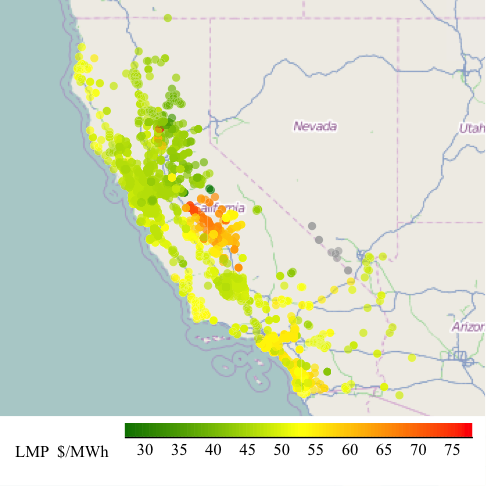
\includegraphics[trim = 0mm 0mm 0mm 0mm, clip, width=0.6\textwidth]{Figures/unprocessed_LMP_map.png}
\caption{Example of Location Marginal Price (LMP) distribution on the CAISO grid. Each circle represents an LMP node on the the CAISO grid. Data from 4PM PDT, August 18 2013}
\label{fig:datamap}
\end{figure}

\section{Results}
In Fig. \ref{fig:chargesize}, \lipsum[66]

\begin{figure}
\centering
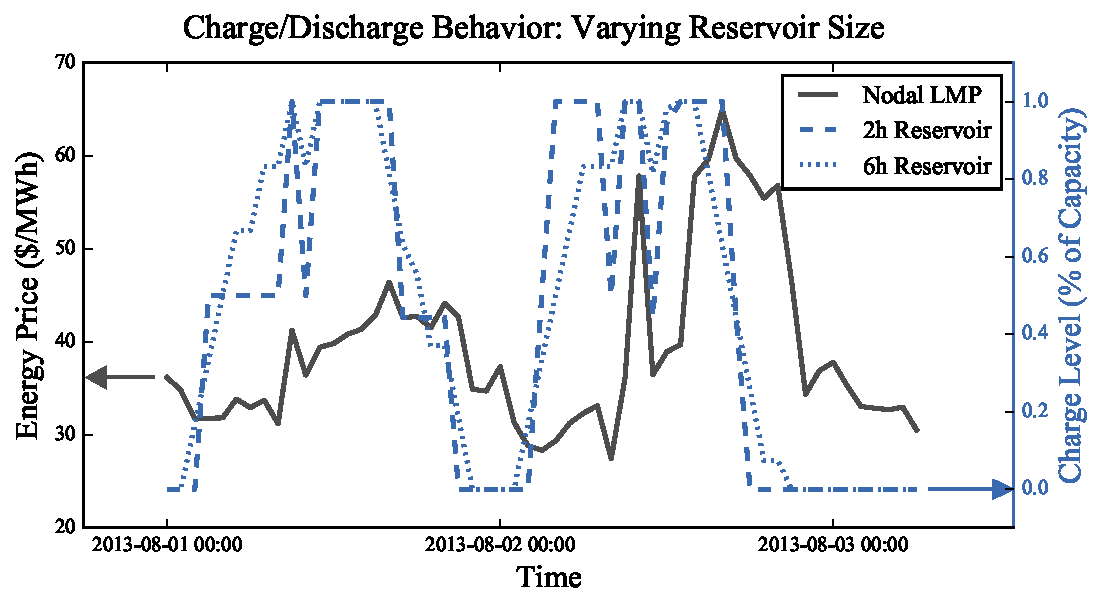
\includegraphics[trim = 0mm 0mm 0mm 0mm, clip, width=0.8\textwidth]{Figures/chargeValidation_varyingSize}
\caption{ Aenean massa. Cum sociis natoque penatibus et magnis dis parturient montes, nascetur ridiculus mus. Donec quam felis, ultricies nec, pellentesque eu, pretium quis, sem. Nulla consequat massa quis enim. }
\label{fig:chargesize}
\end{figure}

\lipsum[2-3]

%%%%%%%%%% CONCLUSION

\section{Conclusion}
\lipsum[22]

\section{Potential Improvements}
\lipsum[5-8]


\chapter{Conclusion}\label{chap:conclusion}
\lipsum[50-53] % Generate paragraphs of random latin text



%%% BIBLIOGRAPHY %%%%%
\bibliographystyle{ieeetr}
\bibliography{chapters/background/APEN_2016_08_02.bib,chapters/blockchains/blockchain.bib}


%%%%%%% APPENDICES - SAME TREATMENT AS ABOVE %%%%%%%%%%
\appendix

%%---------------
\chapter{Decentralized Security- Analytic Solution}
\makeatletter
\def\input@path{{chapters/blockchains/}}
\def\Ginput@path{{chapters/blockchains/}}
\makeatother
\section{Analytic Solution Notes}\label{sec:appendix_analyticSolution}

The x-update step is an unconstrained quadratic program, and can be solved analytically. For clarity, we let $\gamma = Bz^k + u^k$ and proceed as:
\begin{align*}
x^{k+1} &= \text{argmin}_x \quad x^T P x + c^T x + \frac{\rho}{2}||Ax+\gamma||^2_2 \\
x^{k+1} &= \text{argmin}_x \quad x^T P x + c^T x + \frac{\rho}{2}(Ax+\gamma)^T (Ax+\gamma)\\
x^{k+1} &= \text{argmin}_x \quad x^T P x + c^T x + \frac{\rho}{2}(x^T A^T Ax + 2 \gamma^T Ax + \gamma^T \gamma)\\
0 &= \frac{\partial}{\partial x} \left( x^T P x + c^T x + \frac{\rho}{2}(x^T A^T Ax + 2 \gamma^T Ax + \gamma^T \gamma) \right)\\
0 &= 2 P x + c + \rho A^T A x + \rho \gamma^T A\\
0 &= (2P + \rho A^T A)x + c + \rho \gamma^T A \\
x &= (2P + \rho A^T A)^{-1}(-c - \rho \gamma^T A)
\end{align*}

Similarly, the z-update step can be solved analytically by letting $\mu=Ax^{k+1} - c + u^k$ and following a similar process to find:
$$
z^{k+1} = (2Q + \rho B^T B)^{-1} (-d - \rho \mu^T B)
$$

These analytic solutions are used in our implementation to avoid inaccuracies induced from a numeric solution.

\subsection{Comparison with Central Solution}
Because the problem is an unconstrained QP and entries with consensus between a subset of variables, a centralized solution can be computed by composing the cost matrices into a single quadratic problem which can be solved analytically.  This is shown here for the case where $c=0$ and $A$ and $B$ are composed as described above, but also can be computed for other $A,B$.

We break P and Q into sub-matrices dependent on the number of consensus constraints $p$, where $P_{11}, Q_{00} \in \mathbb{R}^{p \times p}$ and the other dimensions follow accordingly.

\begin{align*}
P &= \left[ \begin{array}{cc} P_{00} & P_{01}\\P_{10} & P_{11} \\ \end{array} \right]\\
Q &= \left[ \begin{array}{cc} Q_{00} & Q_{01}\\Q_{10} & Q_{11}\end{array} \right]\\
\Pi &= \left[ \begin{array}{ccc}  P_{00} & P_{01} & 0 \\ P_{10} & P_{11}+Q_{00} & Q_{10} \\
0 & Q_{10} & Q_{11} \end{array} \right]
\end{align*}

Similarly, the $c$ and $d$ vectors can be combined as 
$$
\kappa = \left[ \begin{array}{c} c_0 \\ c_1 + d_0 \\ d_1 \end{array} \right]
$$

The problem can then be expressed as an unconstrained minimization problem:
$$
\text{min}_w \quad w^T \Pi w + \kappa^T w
$$
which is solved by $w^* = -\frac{1}{2}(\Pi^T) ^{-1} \kappa$

This central solution was used only for verification.

%%---------------


\end{document}